\documentclass{beamer}
\usepackage[utf8]{inputenc}
\usetheme{Copenhagen}
\usepackage[spanish]{babel}
\usepackage{multirow}
%\usepackage{estilo-apuntes}
\usepackage[]{graphicx}
\usepackage{svg}

\theoremstyle{definition}

\newtheorem{teorema}{Teorema}
\newtheorem{defi}{Definición}
\newtheorem{prop}[teorema]{Proposición}

\newcommand{\Z}{\mathbb{Z}}
\newcommand{\C}{\mathbb{C}}
\newcommand{\D}{\mathbb{D}}
\providecommand{\gene}[1]{\langle{#1}\rangle}


\addtobeamertemplate{navigation symbols}{}{%
    \usebeamerfont{footline}%
    \usebeamercolor[fg]{footline}%
    \hspace{1em}%
    \insertframenumber/\inserttotalframenumber
}
\setbeamercolor{footline}{fg=black}
\setbeamerfont{footline}{series=\bfseries}

%-----------------------------------------------------------

\title{Modelo basado en arboles}
\author{Alguien}
\institute{Universidad de Sevilla}
\date{}
 
\begin{document}
\frame{\titlepage}
%\begin{frame}
%
%
%\title[About Beamer] %optional
%{About the Beamer class in presentation making}
% 
%\subtitle{A short story}
% 
%\author[Arthur, Doe] % (optional, for multiple authors)
%{A.~B.~Arthur\inst{1} \and J.~Doe\inst{2}}
% 
%\institute[VFU] % (optional)
%{
%  \inst{1}%
%  Faculty of Physics\\
%  Very Famous University
%  \and
%  \inst{2}%
%  Faculty of Chemistry\\
%  Very Famous University
%}
% 
%\date[VLC 2013] % (optional)
%{Very Large Conference, April 2013}


%\end{frame}

%\AtBeginSection[]{
\begin{frame}
\frametitle{Tabla de contenidos}
\tableofcontents
\end{frame}
%}

\section{Estratificación}

\begin{frame}
\begin{figure}[h!]
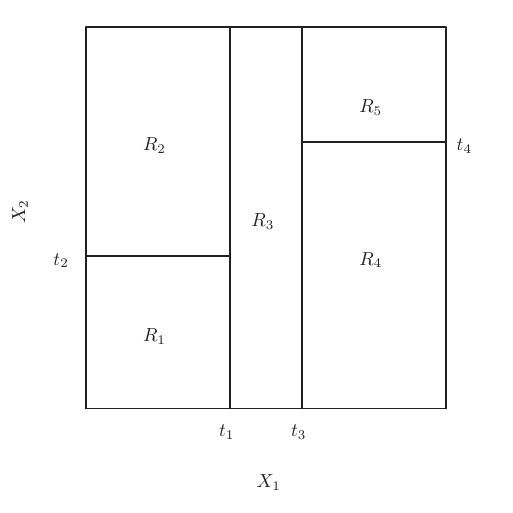
\includegraphics[scale=0.4]{regiones}
\end{figure}
\end{frame}

\begin{frame}
\begin{figure}[h!]
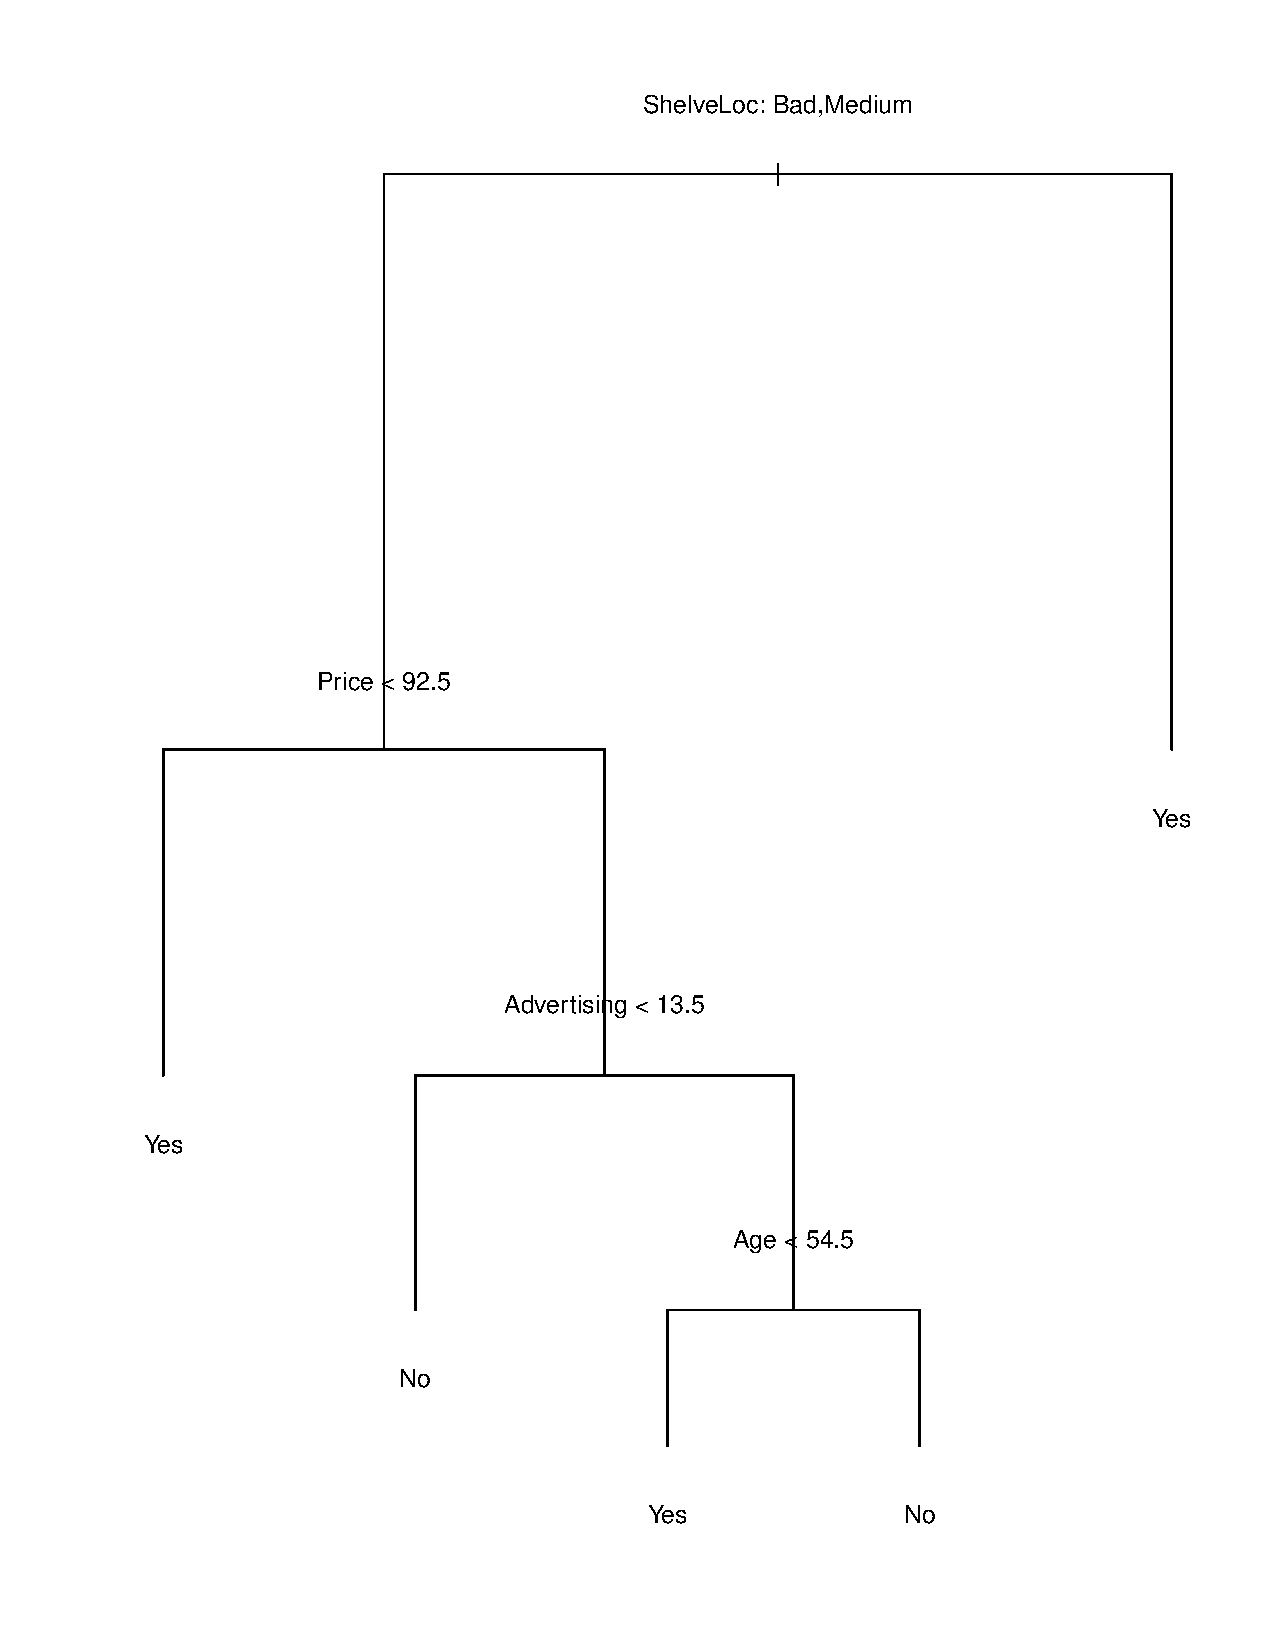
\includegraphics[scale=0.28]{grafo1}
\end{figure}
\end{frame}

\section{Recursive Binary Splitting}
\begin{frame}
\begin{figure}[h!]
\includesvg[scale=0.5]{./dibujo}
\end{figure}
\end{frame}

\begin{frame}
\begin{figure}[h!]
\includesvg[scale=0.5]{./dibujo2}
\end{figure}
\end{frame}

\begin{frame}
\[ \min \sum_{i\colon x_i \in R_1(j,s)} (y_i - \widehat{y}_{R_1})^2 + \sum_{i\colon x_i \in R_2(j,s)} (y_i - \widehat{y}_{R_2})^2 \]
\end{frame}

\begin{frame}
\begin{figure}[h!]
\includesvg[scale=0.5]{./dibujo3}
\end{figure}
\end{frame}


\begin{frame}
\begin{figure}[h!]
\includesvg[scale=0.5]{./dibujo4}
\end{figure}
\end{frame}

\section{Prunning}
\begin{frame}
\begin{figure}[h!]
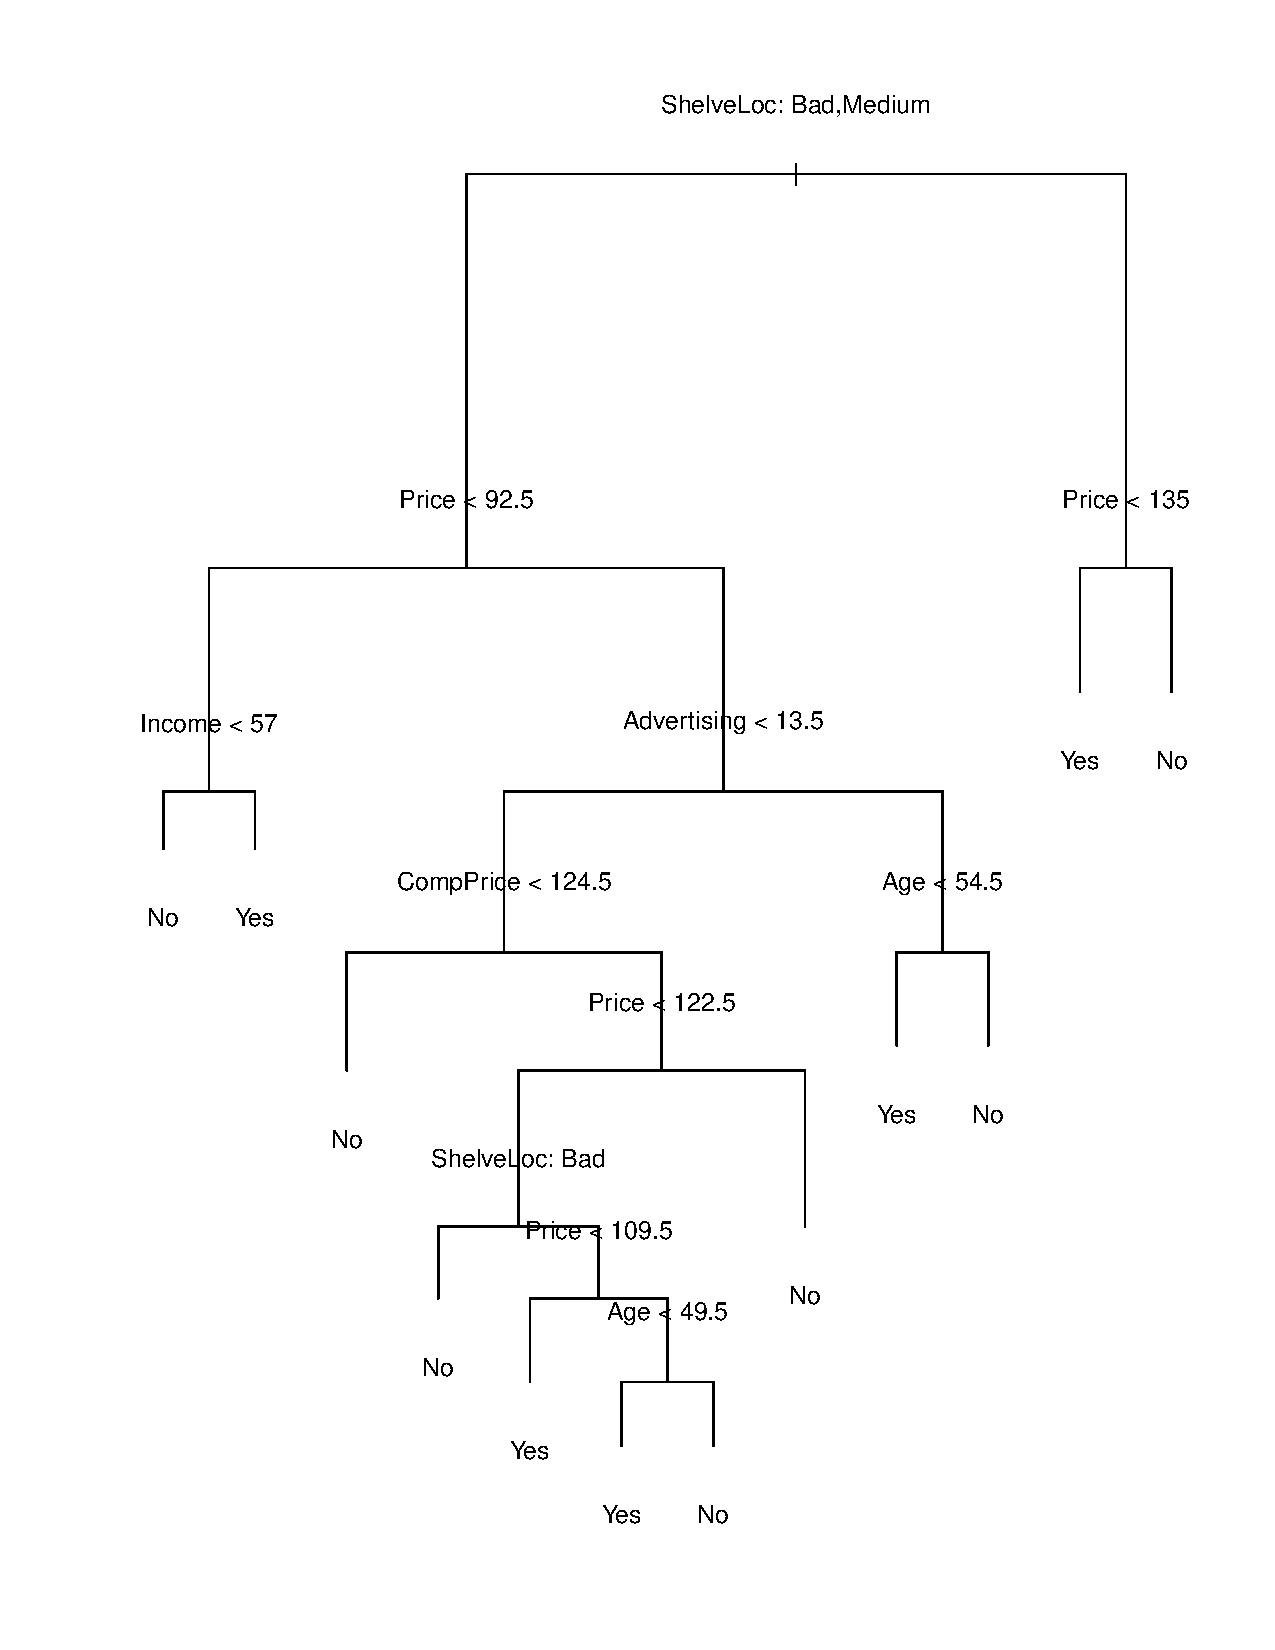
\includegraphics[scale=0.28]{arbolgrande}
\end{figure}
\end{frame}

\begin{frame}
\begin{enumerate}
	\item<1-> Crea un árbol grande $T_0$.
	\item<2-> Para cada valor $\alpha$, encuentra el subarbol $T$ que minimiza
	\[ \sum_{m=1}^{|T|} \sum_{i\colon x_I \in R_m} (y_i - \widehat{y}_{R_m})^2 + \alpha|T| \]
	\item<3-> Use cross-validation para elegir $\alpha$.
	\item<3-> Devuelve su correspondiente árbol.
\end{enumerate}
\end{frame}

\begin{frame}
\begin{figure}[h!]
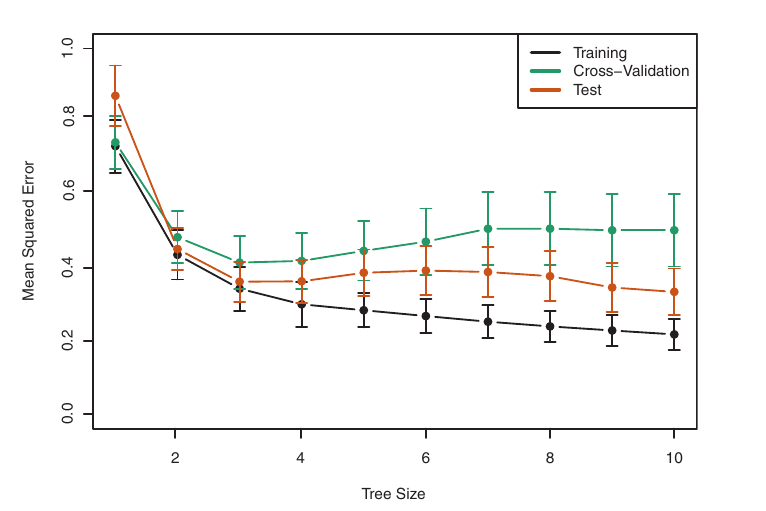
\includegraphics[scale=0.5]{prunning}
\end{figure}
\end{frame}

\begin{frame}
\begin{figure}[h!]
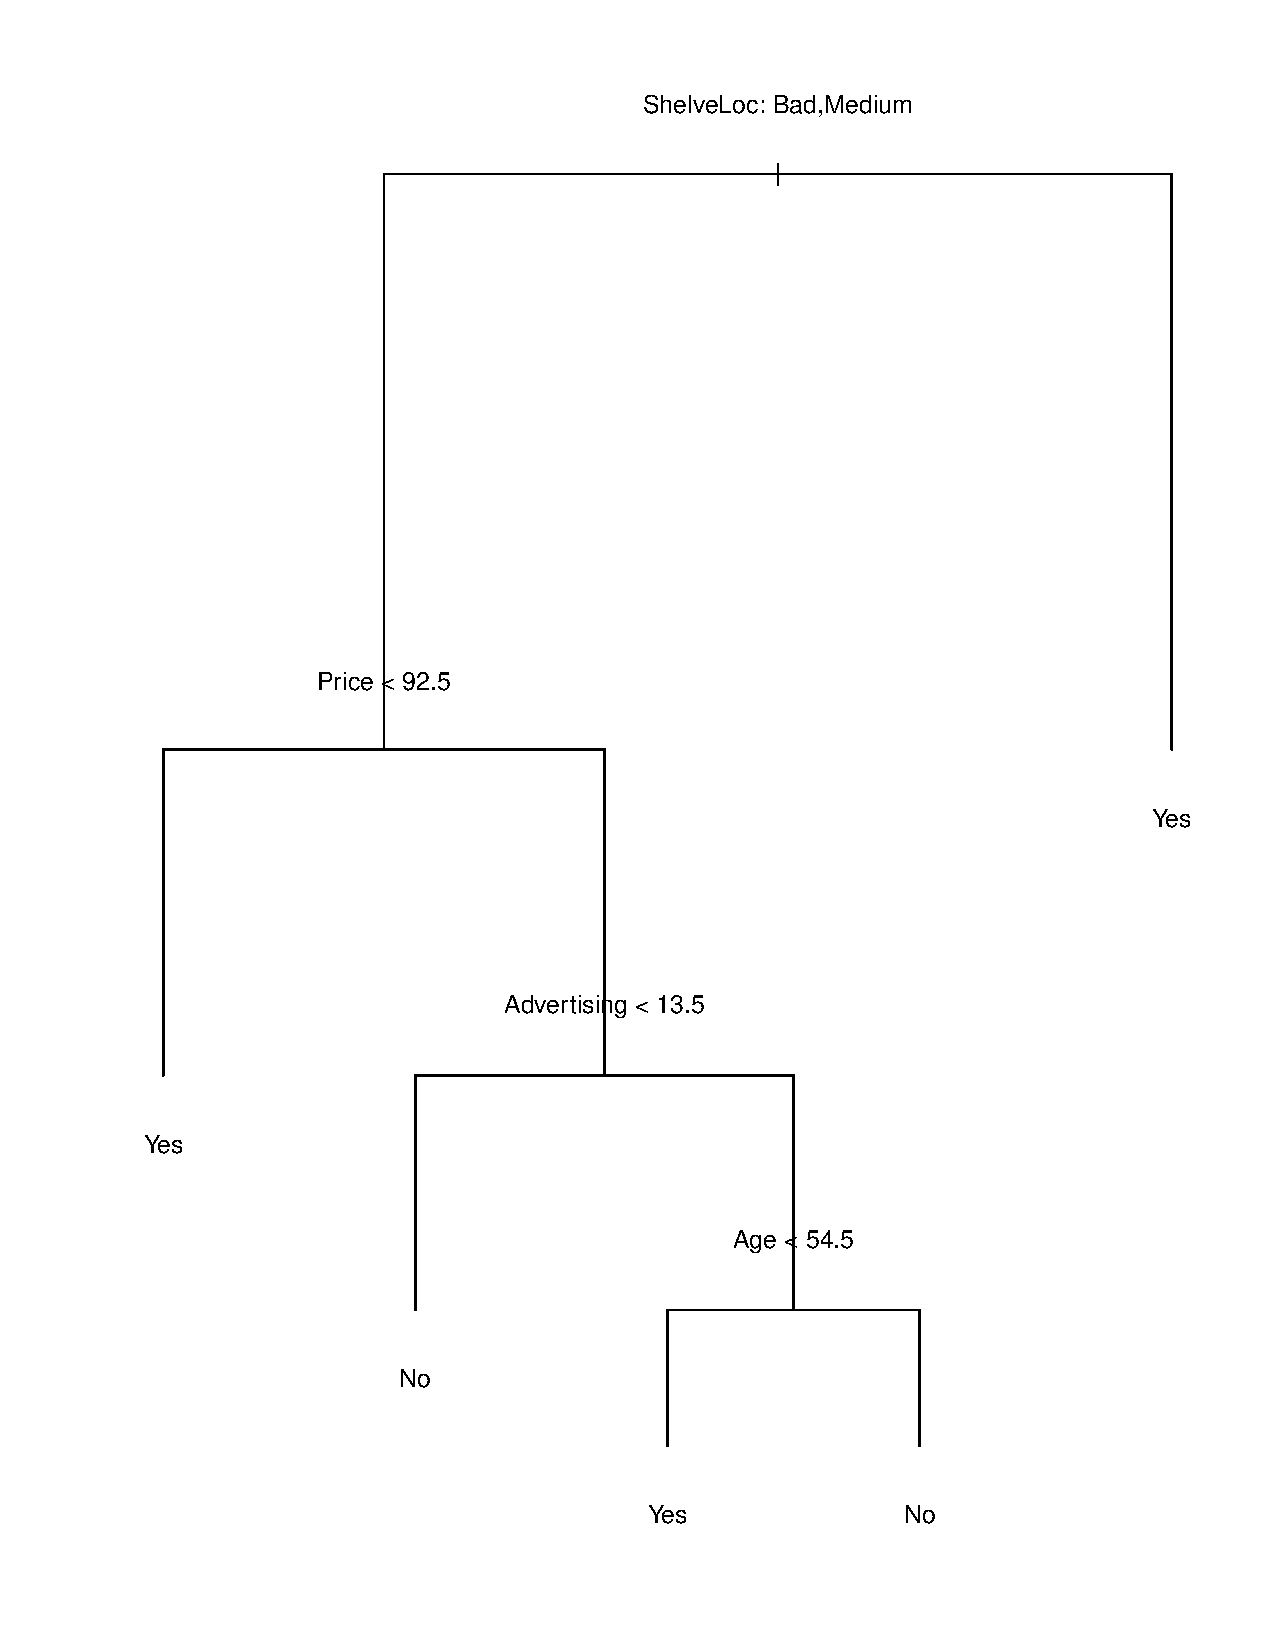
\includegraphics[scale=0.28]{grafo1}
\end{figure}
\end{frame}


\end{document}